% A0 portrait conference poster for Pub_PopInt_PartB (841 x 1189 mm), 2026-09-23.
% Same material as poster_landscape.tex, rearranged: the flow chart runs top to
% bottom in the first column, and the six content blocks sit in a 2 x 3 grid.
% Build:   latexmk -pdf -outdir=out poster_portrait.tex
% Figures: figs/system_pipeline_vertical.pdf (from system_pipeline_vertical.tex),
%          figs/fig4_theta_violin_portrait.pdf (make_poster_figs.py --violin-only).
\documentclass{article}

\usepackage[paperwidth=841mm,paperheight=1189mm,margin=18mm]{geometry}
\usepackage[T1]{fontenc}
\usepackage[utf8]{inputenc}
\usepackage{lato}
% lato.sty (2019) does not set a default family; select it by name, or text falls back to CM Sans.
\renewcommand{\sfdefault}{lato-TLF}
\renewcommand{\familydefault}{\sfdefault}
\usepackage{anyfontsize}
\usepackage{amsmath,amssymb}
\usepackage{booktabs}
\usepackage{graphicx}
\usepackage{xcolor}
\usepackage[most]{tcolorbox}
\usepackage{qrcode}
\usepackage{enumitem}

\definecolor{dtured}{HTML}{990000}
\definecolor{dtugrey}{HTML}{4A4A4A}
\definecolor{dtusand}{HTML}{F7F2EE}

\pagestyle{empty}
\setlength{\parindent}{0pt}
\setlength{\parskip}{0pt}

% ---- type scale (A0, read at 1.5-2 m) ----
\newcommand{\Title}{\fontsize{80}{88}\selectfont}
\newcommand{\Subtitle}{\fontsize{38}{46}\selectfont}
\newcommand{\Byline}{\fontsize{28}{36}\selectfont}
\newcommand{\Author}{\fontsize{46}{54}\selectfont}
\newcommand{\Email}{\fontsize{36}{44}\selectfont}
\newcommand{\Head}{\fontsize{42}{50}\selectfont}
\newcommand{\Body}{\fontsize{34}{44}\selectfont}
\newcommand{\Small}{\fontsize{25}{32}\selectfont}
\newcommand{\Mathsize}{\fontsize{36}{46}\selectfont}

\newtcolorbox{pbox}[2][]{%
  enhanced, colback=white, colframe=dtured, boxrule=1.1mm, arc=3mm,
  title={#2}, fonttitle=\bfseries\Head, coltitle=white, colbacktitle=dtured,
  left=8mm, right=8mm, top=6mm, bottom=6mm, toptitle=3mm, bottomtitle=3mm,
  fontupper=\Body\raggedright, #1}

\setlist[itemize]{leftmargin=11mm, itemsep=5mm, topsep=0mm,
  label={\color{dtured}$\blacktriangleright$}}

% ---- grid: flow column + two content columns, three rows ----
\newlength{\flowcolw}\setlength{\flowcolw}{250mm}
\newlength{\colgap}\setlength{\colgap}{10mm}
\newlength{\colw}\setlength{\colw}{267.5mm}   % (805 - 250 - 2 x 10) / 2
\newlength{\bodyh}\setlength{\bodyh}{1050mm}
\newlength{\rowgap}\setlength{\rowgap}{9mm}
\newlength{\rowA}\setlength{\rowA}{352mm}
\newlength{\rowB}\setlength{\rowB}{362mm}
\newlength{\rowC}\setlength{\rowC}{318mm}      % rowA + rowB + rowC + 2 rowgap = bodyh

\begin{document}

% =====================  HEADER  =====================
\begin{tcolorbox}[enhanced, colback=dtured, colframe=dtured, boxrule=0mm,
  arc=4mm, left=10mm, right=10mm, top=7mm, bottom=7mm, width=\textwidth]
\begin{minipage}[c]{62mm}
  
\includegraphics[height=72mm]{DTU_Logo_White.png}
\end{minipage}\hspace{6mm}%
\begin{minipage}[c]{445mm}
  \color{white}
  {\Title\bfseries From Fractions to Individuals\par}
  \vspace{4mm}
  {\Subtitle Information-Theoretic Integerization for Population Synthesis\par}
  \vspace{4mm}
  {\Byline DTU Management, Transport Division\quad\textbullet\quad
   Technical University of Denmark\par}
\end{minipage}\hfill
\begin{minipage}[c]{150mm}
  \raggedleft\color{white}
  {\Author\bfseries Jeppe Rich\par}
  \vspace{5mm}
  {\Email rich@dtu.dk\par}
\end{minipage}\hspace{8mm}%
\begin{minipage}[c]{58mm}
  \centering
  \colorbox{white}{\qrcode[height=48mm]{https://github.com/jepperich69/Pub_PopInt_PartB}}\par
  \vspace{2mm}
  {\color{white}\Small Code and data\par}
\end{minipage}
\end{tcolorbox}

\vspace{7mm}

\noindent
% =====================  COLUMN 1: PIPELINE  =====================
\begin{minipage}[t][\bodyh][t]{\flowcolw}\vspace{0pt}
\begin{tcolorbox}[enhanced, colback=white, colframe=dtugrey!40, boxrule=0.6mm,
  arc=3mm, left=3mm, right=3mm, top=3mm, bottom=3mm, width=\flowcolw,
  height=\bodyh, valign=center]
\centering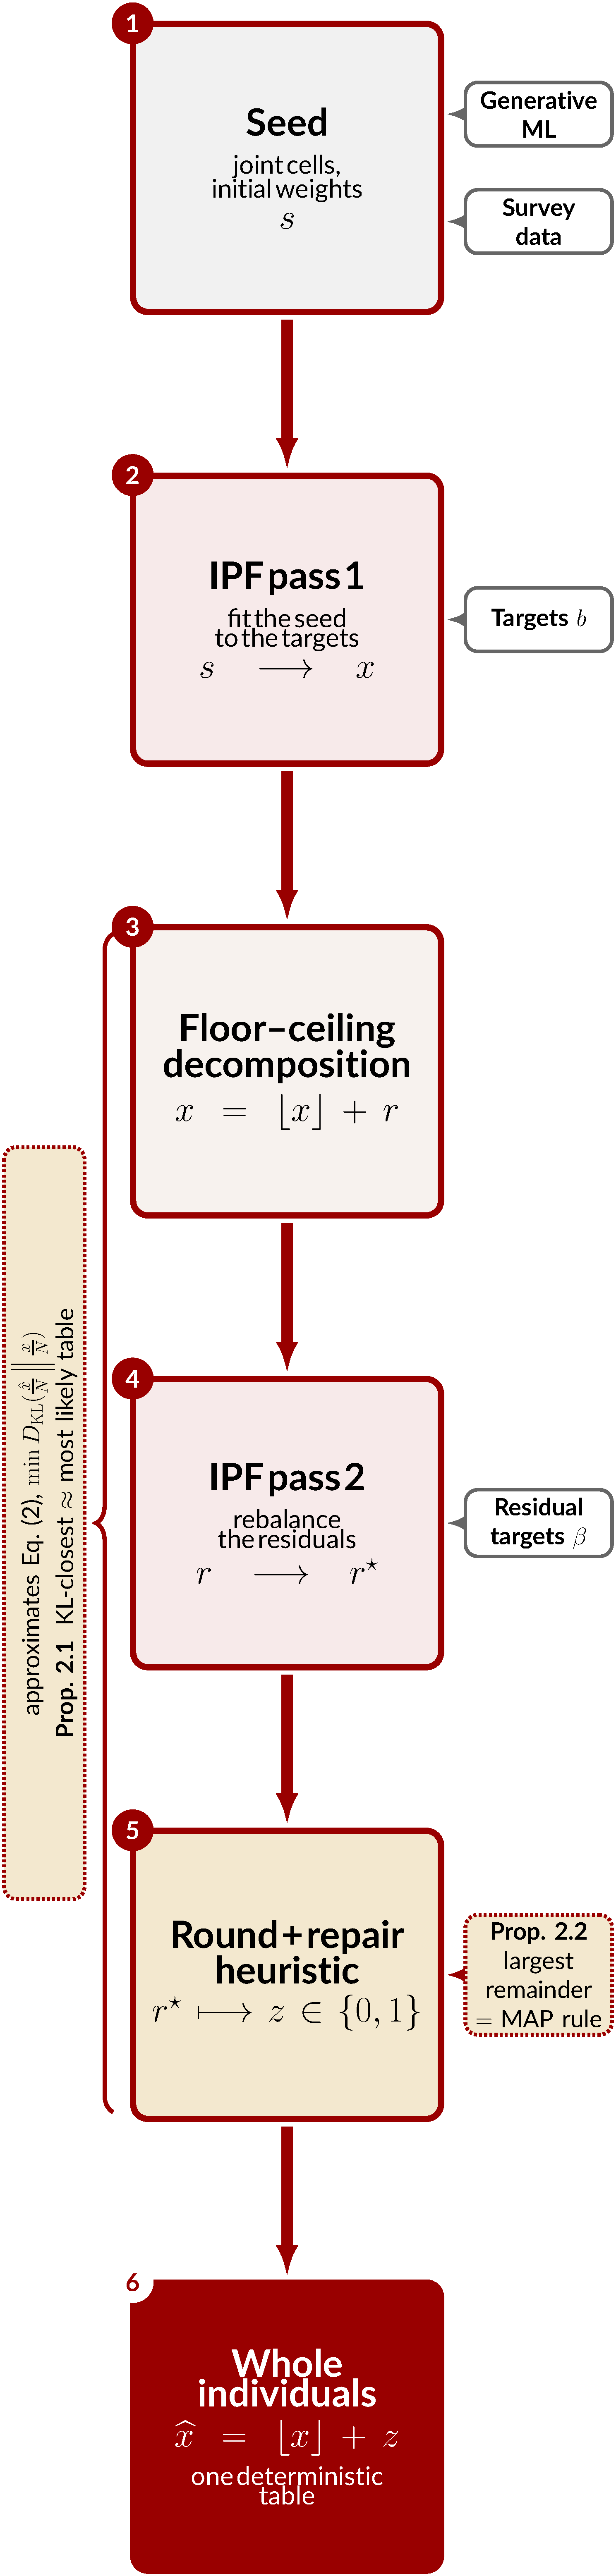
\includegraphics[width=\linewidth,height=\dimexpr\bodyh-8mm\relax,
  keepaspectratio]{figs/system_pipeline_vertical.pdf}
\end{tcolorbox}
\end{minipage}\hspace{\colgap}%
% =====================  COLUMNS 2-3: 2 x 3 GRID  =====================
\begin{minipage}[t][\bodyh][t]{\dimexpr 2\colw+\colgap\relax}\vspace{0pt}
% ---- row 1 ----
\begin{minipage}[t]{\colw}
\begin{pbox}[height=\rowA]{Introduction}
\begin{itemize}
\item Agent-based transport models need whole individuals. The problem grows
      as population tables get sparser, because a large share of the
      population then sits in cells with fractional counts.
\item Uninformed sampling creates two problems: (i) the margins do not hold,
      and (ii) the sampling error is large (Lovelace and Ballas, 2013).
\item In forecasting, a scenario difference should reflect the policy, not
      the random seed.
\item \textbf{Idea:} among all integer tables that meet the margins, choose the
      one closest to the IPF table in KL divergence.
\item Hence, the method extends the KL projection of IPF (Deming and
      Stephan, 1940) to integer allocation, close to the KL optimum.
\end{itemize}
\end{pbox}
\end{minipage}\hfill
\begin{minipage}[t]{\colw}
\begin{pbox}[height=\rowA]{Methodology}
\begin{itemize}[itemsep=2.5mm]
\item \textbf{The problem}, Eq.\ (2):\par
      \vspace{1mm}
      {\centering\fontsize{38}{46}\selectfont
       $\displaystyle\min_{\hat{x}\in\mathbb{Z}_{\ge0}} D_{\mathrm{KL}}\!\left(\frac{\hat{x}}{N}\,\Big\|\,\frac{x}{N}\right)$\\[2mm]
       $\text{s.t.}\quad \sum_{k\in\mathcal{K}(s)}\hat{x}_k=b_s$\par}
\item \textbf{Why hard:} a nonlinear integer program with one variable per cell;
      with overlapping margins it is not guaranteed to be totally unimodular.
\item \textbf{Solution approach:} in the spirit of KL divergence and almost
      optimal, within 3.6\% of the KL optimum.
\end{itemize}
\vspace{2mm}
\begin{tcolorbox}[enhanced, colback=dtusand, colframe=dtured!60, boxrule=0.6mm,
  arc=2mm, left=5mm, right=5mm, top=2mm, bottom=2mm, fontupper=\Body\raggedright]
\begin{itemize}[itemsep=1mm]
\item \textbf{Two passes:} IPF fits the seed, then rebalances the residuals.
\item \textbf{Floor--ceiling:} $\hat{x}=\lfloor x\rfloor+z$, $z\in\{0,1\}$.
\item \textbf{Round + repair:} largest remainder, then $\pm1$ swaps.
\end{itemize}
\end{tcolorbox}
\end{pbox}
\end{minipage}

\vspace{\rowgap}

% ---- row 2 ----
\begin{minipage}[t]{\colw}
\begin{pbox}[height=\rowB]{Application and implications}
\begin{itemize}[itemsep=2.5mm]
\item \textbf{Denmark:} 98 municipalities, 635{,}000 joint cells, 5.9 million persons.
\item \textbf{KL allocation, no noise:} {\color{dtured}\bfseries 98.4\%} of
      the mass in place, against {\bfseries 92.1\%} for multinomial sampling, with zero
      run-to-run variance \textcolor{dtured}{(Fig.\ 5)}.
\item \textbf{Margins:} the controlling targets hold exactly; the secondary
      margins give way, by 1.4\% \textcolor{dtured}{(Table 3)}.
\item \textbf{Scalable:} 397 million cells in 16 minutes; the controlled
      table keeps $\theta_B=0.984$ \textcolor{dtured}{(Table 4)}.
\end{itemize}
\vspace{2mm}
\begin{tcolorbox}[enhanced, colback=dtusand, colframe=dtured!60, boxrule=0.6mm,
  arc=2mm, left=5mm, right=5mm, top=2mm, bottom=2mm, fontupper=\Body\raggedright]
{\bfseries\color{dtured} Implications}\par\vspace{2mm}
\begin{itemize}[itemsep=2mm]
\item No algorithmic sampling noise: scenario differences reflect the policy.
\item 292{,}000 fewer persons misplaced than with multinomial sampling
      (53{,}000 against 345{,}000).
\end{itemize}
\end{tcolorbox}
\end{pbox}
\end{minipage}\hfill
\begin{minipage}[t]{\colw}
\begin{pbox}[height=\rowB, valign=center, left=4mm, right=4mm]{Overlap with the fractional table (Fig.\ 5)}
\centering
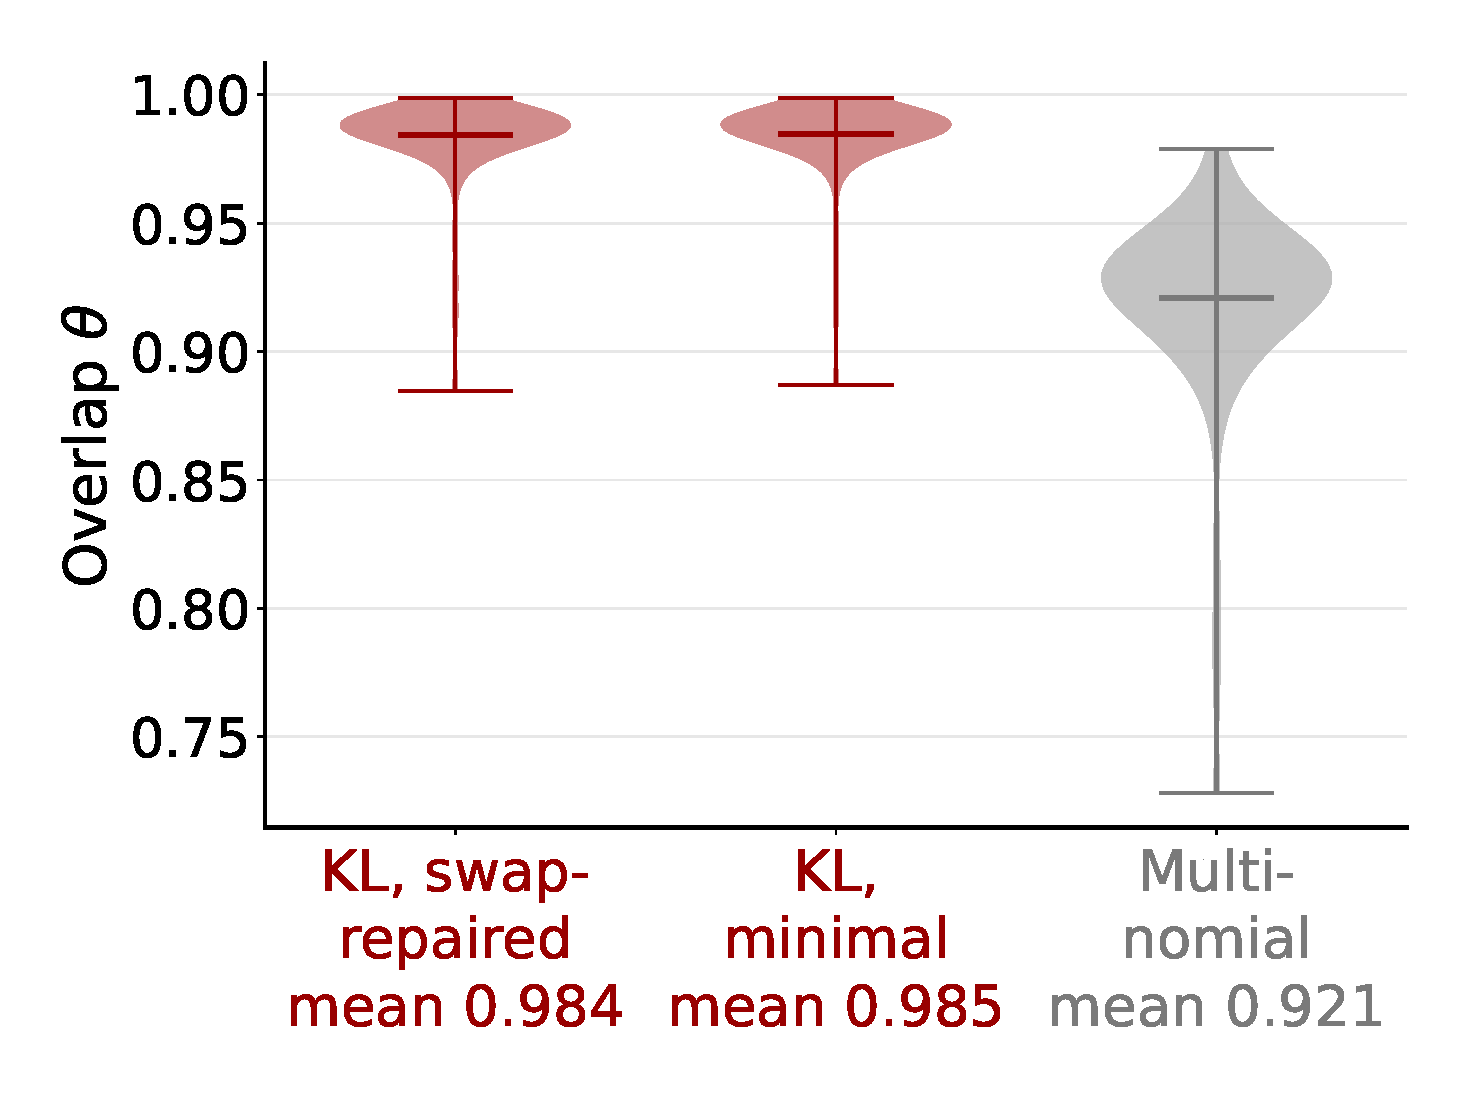
\includegraphics[width=\linewidth]{figs/fig4_theta_violin_portrait.pdf}\par
\vspace{4mm}
{\Body\color{dtugrey} $\theta=\sum_k\min(p_k,q_k)$, 98 municipalities; multinomial: median of 200 draws\par}
\end{pbox}
\end{minipage}

\vspace{\rowgap}

% ---- row 3 ----
\begin{minipage}[t]{\colw}
\begin{pbox}[height=\rowC, valign=center, left=4mm, right=4mm]{Benchmark (Table 3)}
\centering{\Body\bfseries\color{dtured} Approaches without a repair mechanism sacrifice
the target margins\par}
\vspace{8mm}
\centering
\resizebox{\linewidth}{!}{\Small\setlength{\tabcolsep}{2.5mm}\renewcommand{\arraystretch}{1.25}
\begin{tabular}{lccccc}
\toprule
Method & $\theta$ & std & Target & Second. & Rare \\
\midrule
\begin{tabular}[c]{@{}l@{}}\textbf{KL, swap-}\\\textbf{repaired}\end{tabular} & \textbf{0.984} & \textbf{0} & \textbf{0.00} & \textbf{1.39} & \textbf{0.92} \\
Hamilton         & 0.985 & 0      & 0.29 & 1.98 & 0.87 \\
TRS              & 0.977 & 0.0002 & 0.28 & 1.75 & 1.05 \\
Multinomial      & 0.921 & 0.0016 & 1.70 & 8.40 & 1.00 \\
\bottomrule
\end{tabular}}\par
\vspace{8mm}
{\Body\color{dtugrey} Margin errors in \% of population; rare = mass kept
in cells with $x_k<1$\par}
\end{pbox}
\end{minipage}\hfill
\begin{minipage}[t]{\colw}
\begin{pbox}[height=\rowC, valign=center, left=4mm, right=4mm]{Scaling (Table 4)}
\centering{\Body\bfseries\color{dtured} As the table gets sparser, the gap between the
fractional IPF table and any integer table grows\par}
\vspace{8mm}
\centering
\resizebox{0.82\linewidth}{!}{\Small\setlength{\tabcolsep}{4mm}\renewcommand{\arraystretch}{1.2}
\begin{tabular}{rrc|cc}
\toprule
 & & & \multicolumn{2}{c}{full-table $\theta$} \\
$k$ & Cells & Floor & KL & Multin. \\
\midrule
0 & 0.63M & 0.95 & 0.984 & 0.921 \\
1 & 3.2M  & 0.87 & 0.949 & 0.850 \\
2 & 15.9M & 0.73 & 0.880 & 0.741 \\
3 & 79.4M & 0.53 & 0.759 & 0.588 \\
4 & 397M  & 0.31 & 0.592 & 0.413 \\
\bottomrule
\end{tabular}}\par
\vspace{8mm}
{\Body\color{dtugrey} $k$ added attributes. Controlled table: KL 0.984, multinomial 0.921 at every $k$.\par}
\end{pbox}
\end{minipage}
\end{minipage}

\end{document}